\section{Step-by-step instructions to add registration ability to HED services}
\label{annex:service_registration}
\subsection{General knowledge}
\label{General knowledge}
The HED has a brand new self-register ability. If your Service is prepared to co-operate with this mechanism then there will be an InfoRegister connecting to it. There are other, so called InfoRegistrar objects present that are the HED self-register mechanism's active elements communicating with different ISIS clouds. (The InfoRegisterContainter is an instance that connects them, but this is just a good-to-know detail.) The system administrator can connect the Services with ISIS clouds connecting InfoRegisters with InfoRegistrars. The configuration (for example during testing your service) has to cover the both side. (It is possible to connect one InfoRegister to more InfoRegistrars and vice versa. See figure \ref{fig:hed_internal_registration_infrastructure}.)
\begin{figure}[ht]
 \centering{
  \scalebox{0.6}{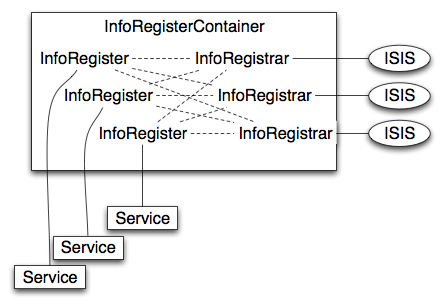
\includegraphics{RegisterRegistrar.png}}
  \caption{\label{fig:hed_internal_registration_infrastructure}The HED internal registration infrastructure}
 }
\end{figure}

The configuration details will be shown on the section Modify your configuration\ref{Modify your configuration}.

The InfoRegistrar that are connected with your Service (by configuration) will periodically ask your Service for a Registration Entry what are stored in the information system. This "poll" is done by executing the RegistrationCollector function that provide an XML document in a given format. For further details see section Compose the Registration Entry\ref{Compose the Registration Entry}! Actually this interface can be accessed in every C++ or Python service.

The InfoRegistrar collect the simultaneous generated Registration Entries and compose a Registration Message by aggregating them (if any aggregation is possible).

The general "sandbox" echo services are already prepared to this functionality and will be referenced at the proper locations.

\subsection{Change your source}
\label{Change your source}

\subsubsection{C++ source}
\label{C++ source}
\begin{itemize}
\item Your Service have to extend the RegisteredService instead of the Service class. This class is implemented in the infosys library and not in the message library as before. (Of course the new library have also to be linked to your Service.)
In your constructor please call the RegisteredService class's constructor!
\item You have also to implement the RegistrationCollector function that will provide the Registration Entry XML document.
\end{itemize}
\textbf{Your\_Service.h}
\begin{verbatim}
...
#include <arc/infosys/RegisteredService.h>
...
class Your_Service: public Arc::RegisteredService {
...
    bool RegistrationCollector(Arc::XMLNode &doc);
...
}
\end{verbatim}
For example see: src/tests/echo/echo.h in the source tree.
\textbf{Your\_Service.cpp}
\begin{verbatim}
...
Your_Service::Your_Service(Arc::Config *cfg):RegisteredService(cfg) {
...
    bool Your_Service::RegistrationCollector(Arc::XMLNode &doc) {
        Arc::NS isis_ns; isis_ns["isis"] = "http://www.nordugrid.org/schemas/isis/2008/08";
        Arc::XMLNode regentry(isis_ns, "RegEntry");
        regentry.NewChild("SrcAdv").NewChild("Type") = "Your_Service_Type";
        regentry.New(doc);
        return true;
    }
...
}
\end{verbatim}
For example see: src/tests/echo/echo.cpp in the source tree.
\textbf{Makefile.am}
\begin{verbatim}
libyourservice_la_LIBADD = ... \
                           $(top_srcdir)/src/hed/libs/infosys/libinfosys.la
\end{verbatim}
For example see: src/tests/echo/Makefile.am in the source tree.

\subsubsection{Python source}
\begin{itemize}
\item The PythonService is already extending the RegisteredService class so you have nothing to do on this place.
\item Your only to-do is to implement the RegistrationCollector function and provide the Registration Entry XML document.
\end{itemize}
\textbf{Your\_Service.py}
\begin{verbatim}
def RegistrationCollector(self, doc):
    regentry = arc.XMLNode('<RegEntry />')
    regentry.NewChild('SrcAdv').NewChild('Type').Set('Your_Service_Type') 
    #Place the document into the doc attribute
    doc.Replace(regentry)
    return True
\end{verbatim}
For example see: src/services/echo\_python/EchoService.py in the source tree.

\subsection{Compose the Registration Entry}
\label{Compose the Registration Entry}
The Registration Entry is an XML document with a given format. The HED internal mechanism tries to aggregate these messages in the Registration Messages.

There are 6 mandatory element in a Registration Entry. At least these should be provided by the service developer. The Type, Endponint reference and the ID of the Service, and the Expiration and Generation time of the message. If the ID is not present then it will be deputized with the Endpoint reference. Finally the Generation time of the message will be also automatically filled if missing from the Registration Entry. (See figure \ref{fig:registration_message}.)
\begin{figure}[ht]
 \centering{
  \scalebox{0.6}{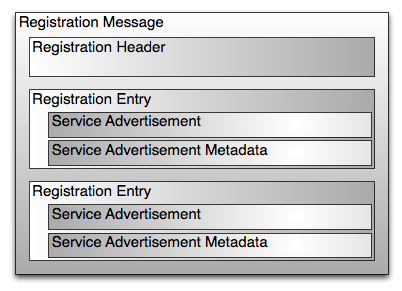
\includegraphics{RegistrationMessage.png}}
  \caption{\label{fig:registration_message}The structure of an aggregated Registration Message}
 }
\end{figure}
The schema of the Registration Entry:
\begin{verbatim}
    <!-- List of the service types will be provided by the GLUE-2.0 -->
    <xsd:simpleType name="ServiceTypeType">
        <xsd:restriction base="xsd:string">
        </xsd:restriction>
    </xsd:simpleType>

    <xsd:complexType name="NameValuePairType">
        <xsd:sequence>
            <xsd:element name="Name" type="xsd:string"/>
            <xsd:element name="Value" type="xsd:string"/>
        </xsd:sequence>
    </xsd:complexType>

    <xsd:complexType name="ServiceAdvertisementMetadataType">
        <xsd:sequence>
            <!-- Globally unique and persistent ID of the service -->
            <xsd:element name="ServiceID" type="xsd:string" minOccurs="1" 
            maxOccurs="1"/>
            <!-- Time of information generation or collection -->
            <xsd:element name="GenTime" type="xsd:dateTime" minOccurs="1" 
            maxOccurs="1"/>
            <xsd:element name="Expiration" type="xsd:duration"/>
        </xsd:sequence>
    </xsd:complexType>

    <xsd:complexType name="ServiceAdvertisementType">
        <xsd:sequence>
            <!-- General part of the Service Advertisment -->
            <xsd:element name="Type" type="isis:ServiceTypeType"/>
            <xsd:element name="EPR" type="wsa:EndpointReferenceType"/>
            <!-- Service specific part of the Service Advertisment -->
            <xsd:element name="SSPair" type="isis:NameValuePairType" minOccurs="0" 
            maxOccurs="unbounded"/>
        </xsd:sequence>
    </xsd:complexType>

    <xsd:complexType name="RegistrationEntryType">
        <xsd:sequence>
            <xsd:element name="SrcAdv" type="isis:ServiceAdvertisementType" 
            minOccurs="1" maxOccurs="1"/>
            <xsd:element name="MetaSrcAdv" type="isis:ServiceAdvertisementMetadataType" 
            minOccurs="1" maxOccurs="1"/>
        </xsd:sequence>
    </xsd:complexType>
\end{verbatim}
It can be also found in the source tree on the path: src/services/isis/schema/isis.xsd
An examle Registration Entry XML document:
\begin{verbatim}
<RegEntry>
  <MetaSrcAdv>
    <ServiceID>http://your.domain.com/echo<ServiceID>
    <GenTime>1994-11-05T13:15:30Z</GenTime>
    <Expiration>PT3H</Expiration>
  </MetaSrcAdv>
  <SrcAdv>
    <Type>org.nordugrid.tests.echo</Type>
    <EPR>
      <Address>http://your.domain.com/echo</Address>
    </EPR>
  </SrcAdv>
</RegEntry>
\end{verbatim}
The service type follows the GLUE2 naming convention and organize the services into categories based on their functionality. The following service types are already defined:

\begin{enumerate}
\item Storage:
\begin{itemize}
\item org.nordugrid.storage.ahash
\item org.nordugrid.storage.bartender
\item org.nordugrid.storage.librarian
\item org.nordugrid.storage.shepherd
\item org.nordugrid.storage.hopi
\end{itemize}
\item Security:
\begin{itemize}
\item org.nordugrid.security.charon
\item org.nordugrid.security.saml
\item org.nordugrid.security.slcs
\item org.nordugrid.security.delegation
\end{itemize}
\item Infosys:
\begin{itemize}
\item org.nordugrid.infosys.isis
\item org.nordugrid.infosys.eils
\item org.nordugrid.infosys.rte-catalog
\end{itemize}
\item Execution:
\begin{itemize}
\item org.nordugrid.execution.arex
\item org.nordugrid.execution.janitor
\item org.nordugrid.execution.sched
\item org.nordugrid.execution.paul
\end{itemize}
\item Accounting:
\begin{itemize}
\item org.nordugrid.accounting.mars
\end{itemize}
\item Tests:
\begin{itemize}
\item org.nordugrid.tests.echo
\item org.nordugrid.tests.echo\_java
\item org.nordugrid.tests.echo\_python
\item org.nordugrid.tests.isistest
\end{itemize}
\end{enumerate}

\subsection{Modify your configuration}
\label{Modify your configuration}
The configuration have to contain the connection between the InfoRegisters (Services) and InfoRegistrars (ISIS clouds). The schema of the configuration can be also found in the source tree (src/hed/libs/infosys/InfoRegisterConfig.xsd). There is also an example configuration between the configuration templates in the source tree (src/hed/profiles/SecureP2PIIS/SecureP2PIIS.xml).

The Service configuration should contain the InfoRegister and implicitly the InfoRegistrar configuration.
\begin{verbatim}
           <infosys:InfoRegister>
	                <infosys:Period>PT20S</infosys:Period>
	                <infosys:Endpoint>https://localhost:50000/example_service</infosys:Endpoint>
	                <infosys:Expiration>PT100S</infosys:Expiration>
	                <infosys:Registrar>
	                    <infosys:URL>some_url</infosys:URL>
	                    <infosys:KeyPath>some_local_path</infosys:KeyPath>
	                    <infosys:CertificatePath>some_local_path</infosys:CertificatePath>
	                    <infosys:CACertificatesDir>some_local_path</infosys:CACertificatesDir>
	                </infosys:Registrar>
	                <infosys:Registrar>
	                    <infosys:URL>	some_other_url</infosys:URL>
	                    <infosys:KeyPath>some_local_path</infosys:KeyPath>
	                    <infosys:CertificatePath>some_local_path</infosys:CertificatePath>
	                    <infosys:CACertificatesDir>some_local_path</infosys:CACertificatesDir>
	                </infosys:Registrar>
	            </infosys:InfoRegister>
\end{verbatim}
If the same InfoRegistrar would exist at more then one Serivce (the URL have to be the same) then the internal HED mechanism detect the similarity and tries to aggregate the messages if it's possible. You can also override the default Period, Endpoint, Expiration values inside the single Registrar elements and them too by written some value in the document in your source.

If the service configuration contains a \begin{verbatim}<NoRegister />\end{verbatim} element then it won't be registered.
